\documentclass[11pt,english]{article}



\listfiles
\usepackage{fullpage}
\usepackage[showframe=false,margin=1in]{geometry}
\parindent=0pt

\usepackage{relsize}
\usepackage[T1]{fontenc} % for properly hyphenating words with accented chars
\usepackage{babel}

\usepackage{epsfig}
\usepackage{graphicx}
\usepackage{wrapfig}
\usepackage[belowskip=0pt,aboveskip=0pt,font=small]{caption}
\usepackage{subcaption}
\setlength{\intextsep}{7pt plus 0pt minus 0pt}

\usepackage{amsmath, amsthm, amssymb}
\usepackage{textcomp}
\usepackage{stmaryrd}
\usepackage{upgreek}
\usepackage{bm}
\usepackage{cases}
\usepackage{mathtools}

\usepackage{url}
\usepackage{breakurl}
\usepackage[colorlinks=true]{hyperref}
\usepackage{xspace}
\usepackage{comment}
\usepackage{color}
\usepackage{afterpage}
\usepackage[normalem]{ulem}
\usepackage{enumitem}




\usepackage{../assets/mysymbols}
\usepackage{amsmath,amsfonts}
\usepackage{amsthm,amssymb,amsopn}
\usepackage{bm} % bold symbol
\usepackage{bbm}
\usepackage{tikz}
\usetikzlibrary{shapes.geometric, arrows.meta, positioning}

\newcommand{\vct}[1]{\boldsymbol{#1}} % vector
\newcommand{\mat}[1]{\boldsymbol{#1}} % matrix

\newcommand{\field}[1]{\mathbb{#1}}
\newcommand{\R}{\field{R}} % real domain
\newcommand{\C}{\field{C}} % complex domain
\newcommand{\F}{\field{F}} % functional domain
\newcommand{\T}{^{\textrm T}} % transpose
\newcommand{\TN}{^{-\textrm T}} % transpose
\newcommand{\Lagr}{\mathcal{L}}


\newcommand{\cst}[1]{\mathsf{#1}}

\newcommand{\inner}[2]{#1\cdot #2}
\newcommand{\twonorm}[1]{\|#1\|_2^2}
\newcommand{\Map}[1]{\mathcal{#1}}

\newcommand{\ProbOpr}[1]{\mathbb{#1}}
\newcommand\independent{\protect\mathpalette{\protect\independenT}{\perp}}
\def\independenT#1#2{\mathrel{\rlap{$#1#2$}\mkern2mu{#1#2}}}
\newcommand{\cind}[3]{{#1} \independent{#2}\,|\,#3}
\newcommand{\cndexp}[2]{\ProbOpr{E}\,[ #1\,|\,#2\,]}



\newtheorem{thm}{Theorem}

\newcommand{\eat}[1]{}

\newcommand{\hide}[1]{}

\newcommand{\diff}{\mathop{}\!\mathrm{d}}
\newcommand{\Vop}{\textrm{T}}
\newcommand{\norminf}[1]{\norm{#1}_\infty}

\newcommand{\vecy}{\ensuremath{\mathbf{y}}\xspace}
\newcommand{\vecx}{\ensuremath{\mathbf{x}}\xspace}
\renewcommand{\argmax}{\operatornamewithlimits{argmax}}
\newcommand{\startsym}{\mbox{\scriptsize \texttt{<s>}}\xspace}
\newcommand{\stopsym}{\mbox{\scriptsize \texttt{</s>}}\xspace}
\newcommand{\best}{\ensuremath{\mathit{best}}\xspace}
\newcommand{\bestuptoi}{\ensuremath{\texttt{best}_{\leq i}}\xspace}
\newcommand{\bestuptot}{\ensuremath{\texttt{best}_{\leq t}}\xspace}
\newcommand{\completed}{\ensuremath{\texttt{comp}}\xspace}
\newcommand{\toptop}{\operatornamewithlimits{\mathbf{top}}}
\newcommand{\tuple}[1]{\ensuremath{\langle {#1} \rangle}}
\newcommand{\xuptot}{\ensuremath{\mathit{x}_{\leq t}}\xspace}


\renewcommand{\hide}[1]{}
\usepackage{graphicx}
\begin{document}
\title{CS 4644/7643: Deep Learning\\
Fall 2026 \\
Problem Set 1}

\author{Instructor: Danfei Xu \\
TAs: Rohan Bansal, Uzu (Chris) Lee, Alfred Cueva  \\
Kun-Lin Hsieh, Chuye Zhang, Liqian Ma, Robert Azarcon  \\
Dhruv Ahuja, Xinchen Yin \\
Discussions: \url{https://piazza.com/class/ms43b2tjxa63lq\#}}
\maketitle

\begin{center}
    \textbf{Student Name:} Venkata Aashutosh Aripirala \quad \textbf{GT Email:} av84@gatech.edu \quad \textbf{GT ID:} 904173725
\end{center}

\paragraph*{Instructions}
\begin{enumerate}
\item We will be using Gradescope to collect your assignments. Please read the following instructions for submitting to Gradescope carefully!
     \begin{itemize}
          \item
               For the \textbf{HW1 Theory} component on Gradescope, upload one single PDF containing the answers to all the theory questions. \textbf{However, the solution to each problem/subproblem must be on a separate page. When submitting to Gradescope, please make sure to mark the page(s) corresponding to each problem/sub-problem.}
          \item
               For the \textbf{HW1 Coding} component on Gradescope, please use the \texttt{collect\_submission.py} script provided and upload the resulting \textbf{hw1\_code\_submission.zip} on Gradescope. Please make sure you have saved the most recent version of your code.
          \item
               For the \textbf{HW1 Notebook} component on Gradescope, please use the \texttt{collect\_submission.py} script provided and upload the resulting \textbf{hw1\_notebook\_submission.pdf} on Gradescope.
          \item
               Note: This is a large class and Gradescope's assignment segmentation features are essential.
               Failure to follow these instructions may result in parts of your assignment not being graded.
               We will not entertain regrading requests for failure to follow instructions.
     \end{itemize}

\item
     \LaTeX'd solutions are strongly encouraged (solution template is provided in hw1\_overleaf.zip), but scanned handwritten copies are acceptable. Hard copies are \textbf{not} accepted.


\item We generally encourage you to collaborate with other students.

You may talk to a friend,
discuss the questions and potential directions for solving them. However, you need to write
your own solutions and code separately, and \emph{not} as a group activity.
Please list the students you collaborated with. \\ \\

\end{enumerate}
\newpage


\section{Collaborators [0.5 points]}

Please list your collaborators and assign this list to the corresponding section of the outline on Gradescope. If you don't have any collaborators, please write 'None' and assign it to the corresponding section of the Gradescope submission regardless. Not assigning this question on Gradescope or leaving it blank will be marked as zero.

\paragraph{Solution:}
None

\newpage

\section{Optimization}

\begin{enumerate}

\item
\textbf{[3 points]}
Let $f(\mathbf{x})$ be a function, where $\mathbf{x} \in \mathbb{R}^d$.
The \textit{level surface} of a function is the set of points with the same value of function, \ie
\begin{equation}
    L_c = \left\{ \mathbf{x} \mid f(\mathbf{x}) = c \right\} \label{q11.ls}
\end{equation}
for some c $\in$ $\mathbb{R}$. 

\begin{figure}[h!]
    \centering
    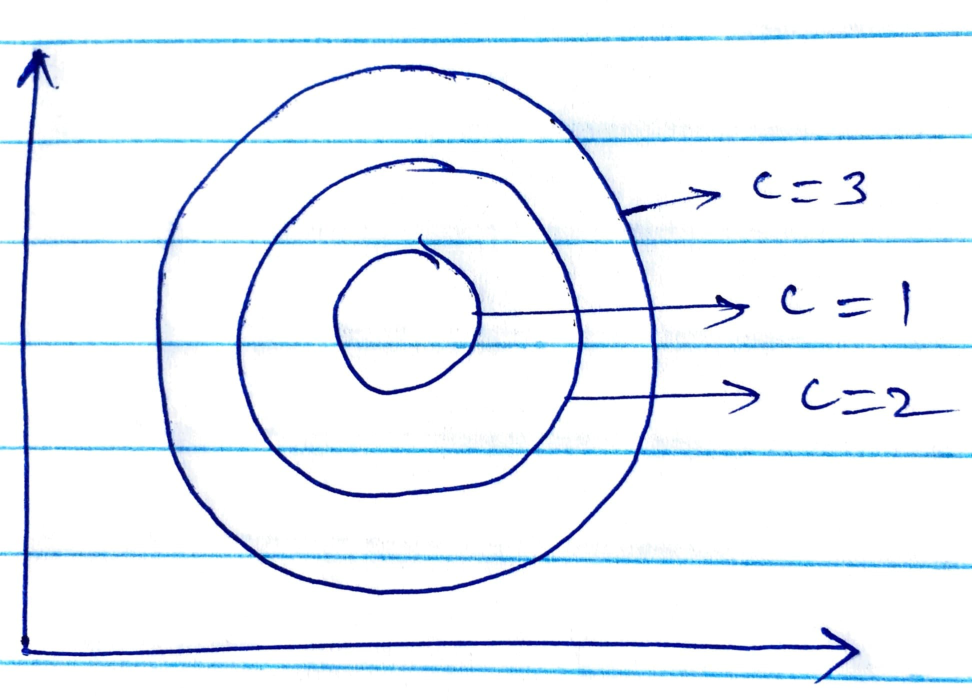
\includegraphics[scale=0.5]{assets/circle_dl.pdf}
\end{figure}

The above figure shows level surfaces for different values of c for a 2-dimensional case. The points on the perimeter of each curve illustrate the set of points sharing the same value, i.e. $f(x_1, x_2) = c$.

Recall that a gradient vector is defined as $\nabla f = \left[ \frac{\partial f}{\partial x_1}, \frac{\partial f}{\partial x_2}, ..., \frac{\partial f}{\partial x_d} \right]$.

Consider a specific point $\mathbf{x}_0 \in \mathbb{R}^d$. Let us denote the level surface passing through this point by $L_{f(\mathbf{x_0})}$. Let us denote the gradient vector at $\mathbf{x_0}$ by $\nabla f_0$. 

Now, consider an arbitrary curve $\mathbf{r}(t) = \left[x_1(t); x_2(t); \ldots, x_d(t)\right]$ (parameterized by a scalar $t$) that passes through $\mathbf{x}_0$, 
\ie $\mathbf{r}(t_0) = \mathbf{x_0}$ for some $t_0 \in \mathbb{R}$. Furthermore, 
the curve $\mathbf{r}(t)$ lies within the level surface passing through $\mathbf{x}_0$, \ie $\mathbf{r}(t) \in L_{f(\mathbf{x_0})}, \,\, \forall t$.  

Recall that the \emph{tangent} to a curve is defined as $\frac{\del \mathbf{r}}{\del t}$. 

With all that context and notation behind us, now comes the `fun' part -- 
show that $\nabla f_0$ is orthogonal to the tangent of $\mathbf{r}(t)$ at $t_0$. 

Now, please describe in non-technical language what you have just proven. Why might we care about this in the context of deep learning? 

\paragraph{Solution:}

\textbf{1. Proof of Orthogonality:}

Since the curve $\mathbf{r}(t)$ is entirely contained within the level surface $L_{f(\mathbf{x}_0)}$ for all $t$, the value of the function $f$ evaluated along the trajectory of the curve is constant:
\begin{equation}
    f(\mathbf{r}(t)) = c = f(\mathbf{x}_0) \quad \forall t
\end{equation}
Differentiating both sides with respect to the scalar parameter $t$:
\begin{equation}
    \frac{\diff}{\diff t} \left[ f(\mathbf{r}(t)) \right] = \frac{\diff}{\diff t}[c] = 0
\end{equation}
Applying the multivariable chain rule to the left-hand side:
\begin{equation}
    \frac{\diff}{\diff t} \left[ f(\mathbf{r}(t)) \right] = \sum_{i=1}^d \frac{\partial f}{\partial x_i}(\mathbf{r}(t)) \frac{\diff x_i}{\diff t}(t) = \nabla f(\mathbf{r}(t)) \cdot \frac{\diff \mathbf{r}}{\diff t}(t) = 0
\end{equation}
Evaluating this expression at $t = t_0$, where $\mathbf{r}(t_0) = \mathbf{x}_0$ and $\nabla f(\mathbf{r}(t_0)) = \nabla f(\mathbf{x}_0) = \nabla f_0$:
\begin{equation}
    \nabla f_0 \cdot \frac{\diff \mathbf{r}}{\diff t}(t_0) = 0
\end{equation}
Since the inner product (dot product) between the gradient vector $\nabla f_0$ and the tangent vector $\frac{\diff \mathbf{r}}{\diff t}(t_0)$ is zero, $\nabla f_0$ is orthogonal (perpendicular) to the tangent vector of any curve lying on the level surface at $\mathbf{x}_0$. $\blacksquare$

\vspace{0.5em}
\textbf{2. Non-Technical Interpretation \& Importance in Deep Learning:}

\begin{itemize}
    \item \textbf{Non-Technical Interpretation:} A level surface (analogous to a contour line on a topographical elevation map) connects all points that share the exact same height or function value. Moving along a level surface yields zero rate of change in the function. The proof demonstrates that the gradient vector points in a direction that is strictly perpendicular (at a $90^\circ$ angle) to these contour lines. Geometrically, this means the gradient points directly away from the path of zero change, pointing along the direction of \emph{steepest ascent} (maximum increase).
    \item \textbf{Why We Care in Deep Learning:} In deep learning, training a neural network corresponds to minimizing a high-dimensional loss surface $L(\mathbf{W})$ over model weights $\mathbf{W}$. Because the gradient $\nabla L(\mathbf{W})$ is perpendicular to the contours of equal loss, the negative gradient $-\nabla L(\mathbf{W})$ points in the direction of \emph{steepest descent}. First-order optimization algorithms such as Gradient Descent, SGD, Momentum, and Adam rely fundamentally on this geometric property to efficiently navigate across the loss surface toward a local or global minimum.
\end{itemize}

\newpage

\item
\textbf{[2 points]}

The softmax function $\mathbf{s}(\mathbf{z})$, which takes a vector input $\mathbf{z}$ and outputs a vector whose $i$th entry $s_i$ is

\begin{equation}
s_i = \frac{e^{z_{i}}}{\sum_{k} e^{z_{k}}}
\end{equation}

The input vector $\mathbf{z}$ to $\mathbf{s}(\cdot)$ is sometimes called the ``logits'', which just means the unscaled output of previous layers. Derive the gradient of $\mathbf{s}$ with respect to the logits, \ie derive $\frac{\partial \mathbf{s}}{\partial \mathbf{z}}$. 

\paragraph{Solution:}

Let $\mathbf{z} = [z_1, z_2, \dots, z_K]^T \in \mathbb{R}^K$ and let $\Sigma = \sum_{k=1}^K e^{z_k}$. The $i$-th component of the softmax function is $s_i = \frac{e^{z_i}}{\Sigma}$.

We wish to compute the Jacobian matrix $\frac{\partial \mathbf{s}}{\partial \mathbf{z}} \in \mathbb{R}^{K \times K}$, whose $(i, j)$-th entry is $\frac{\partial s_i}{\partial z_j}$. Applying the quotient rule:
\begin{equation}
    \frac{\partial s_i}{\partial z_j} = \frac{\frac{\partial (e^{z_i})}{\partial z_j} \Sigma - e^{z_i} \frac{\partial \Sigma}{\partial z_j}}{\Sigma^2}
\end{equation}
We evaluate the partial derivatives involved:
\begin{align}
    \frac{\partial (e^{z_i})}{\partial z_j} &= \begin{cases} e^{z_i} & \text{if } i = j \\ 0 & \text{if } i \neq j \end{cases} = \delta_{ij} e^{z_i} \\
    \frac{\partial \Sigma}{\partial z_j} &= \frac{\partial}{\partial z_j} \left( \sum_{k=1}^K e^{z_k} \right) = e^{z_j}
\end{align}
where $\delta_{ij}$ is the Kronecker delta ($\delta_{ij} = 1$ if $i = j$, and $\delta_{ij} = 0$ if $i \neq j$).

Substituting these back into the quotient rule:
\begin{align}
    \frac{\partial s_i}{\partial z_j} &= \frac{\delta_{ij} e^{z_i} \Sigma - e^{z_i} e^{z_j}}{\Sigma^2} \\
    &= \delta_{ij} \frac{e^{z_i}}{\Sigma} - \left(\frac{e^{z_i}}{\Sigma}\right) \left(\frac{e^{z_j}}{\Sigma}\right) \\
    &= \delta_{ij} s_i - s_i s_j \\
    &= s_i (\delta_{ij} - s_j)
\end{align}

Explicitly written for the diagonal and off-diagonal elements:
\begin{equation}
    \frac{\partial s_i}{\partial z_j} = \begin{cases} 
    s_i (1 - s_i) & \text{if } i = j \\ 
    -s_i s_j & \text{if } i \neq j 
    \end{cases}
\end{equation}

In compact matrix notation, the Jacobian matrix is given by:
\begin{equation}
    \frac{\partial \mathbf{s}}{\partial \mathbf{z}} = \operatorname{diag}(\mathbf{s}) - \mathbf{s} \mathbf{s}^T
\end{equation}
where $\operatorname{diag}(\mathbf{s})$ is the $K \times K$ diagonal matrix containing vector $\mathbf{s}$ on its diagonal.

\newpage

\item
\textbf{[3 points: Extra credit for both 4644 and 7643]}

Recall that a ($d-1$)-dimensional simplex is defined as: 
\begin{equation}
    \Delta_{d - 1} = \{\mathbf{p} \in \mathbb{R}^{d} \mid \mathbf{1}^{T}\mathbf{p} = 1 \text{ and } p_i \ge 0 \,\, \forall i \in \{1,\ldots,d\} \}
\end{equation}

In this question, you will develop an interpretation of softmax as a projection operator -- that it projects an arbitrary point $\mathbf{x} \in \mathbb{R}^d$ onto the interior of the $d - 1$ simplex. Specifically, let $\mathbf{s}(\mathbf{x})$ denote the softmax function (as defined above). Now prove that, 


\begin{align}
    \mathbf{s}(\mathbf{x}) =  \argmin_{\mathbf{y} \in \mathbb{R}^d} &\quad  -\mathbf{x}^{T}\mathbf{y} - H(\mathbf{y}) \\ 
     \st & \quad \mathbf{1}^{T}\mathbf{y} = 1, \quad 0 \le y_i \le 1 \quad \forall i
\end{align}

where $H$ is the entropy function: 

\begin{equation}
    H(\mathbf{y}) = - \sum_{i}y_{i}\log(y_{i})
\end{equation}

Now, what does this formal interpretation tell you about the softmax layer in a neural network? 
Hint: Look at the KKT conditions.

\paragraph{Solution:}

\textbf{1. Proof via KKT Conditions:}

We consider the constrained optimization problem:
\begin{equation}
    \min_{\mathbf{y} \in \mathbb{R}^d} f(\mathbf{y}) = -\mathbf{x}^T \mathbf{y} - H(\mathbf{y}) = -\sum_{i=1}^d x_i y_i + \sum_{i=1}^d y_i \ln y_i
\end{equation}
subject to:
\begin{align}
    h(\mathbf{y}) &= \sum_{i=1}^d y_i - 1 = 0 \\
    g_{1, i}(\mathbf{y}) &= -y_i \le 0, \quad \forall i \in \{1, \dots, d\} \\
    g_{2, i}(\mathbf{y}) &= y_i - 1 \le 0, \quad \forall i \in \{1, \dots, d\}
\end{align}

The objective function $f(\mathbf{y})$ is strictly convex on the interior of the simplex because the negative entropy function $-H(\mathbf{y}) = \sum_i y_i \ln y_i$ is strictly convex on $(0, 1]^d$ (its Hessian $\nabla^2 (-H(\mathbf{y})) = \operatorname{diag}(1/y_1, \dots, 1/y_d)$ is strictly positive definite for $y_i > 0$), and $-\mathbf{x}^T \mathbf{y}$ is linear. Since the constraints are affine, Slater's condition is satisfied, and the KKT conditions are both necessary and sufficient for the unique global optimum $\mathbf{y}^*$.

Furthermore, notice that $\lim_{y_i \to 0^+} \frac{\diff}{\diff y_i}(y_i \ln y_i) = \lim_{y_i \to 0^+} (\ln y_i + 1) = -\infty$. Consequently, any boundary point where $y_i = 0$ would cause the directional derivative outward from the boundary to be $-\infty$, pulling the solution strictly into the interior $y_i > 0$. Therefore, the optimal solution lies strictly in the relative interior of the simplex: $0 < y_i < 1$ for all $i$.

By complementary slackness, the inequality multipliers associated with $-y_i \le 0$ and $y_i \le 1$ are zero ($\mu_i = 0, \nu_i = 0, \forall i$).

The Lagrangian with equality multiplier $\lambda \in \mathbb{R}$ is:
\begin{equation}
    \mathcal{L}(\mathbf{y}, \lambda) = \sum_{i=1}^d (y_i \ln y_i - x_i y_i) + \lambda \left(\sum_{i=1}^d y_i - 1\right)
\end{equation}
Setting the partial derivative of $\mathcal{L}$ with respect to each $y_i$ to zero (stationarity condition):
\begin{equation}
    \frac{\partial \mathcal{L}}{\partial y_i} = \ln y_i + 1 - x_i + \lambda = 0
\end{equation}
Solving for $y_i$:
\begin{align}
    \ln y_i &= x_i - 1 - \lambda \\
    y_i &= e^{x_i - 1 - \lambda} = e^{-(1+\lambda)} e^{x_i}
\end{align}
Using the probability normalization constraint $\sum_{i=1}^d y_i = 1$:
\begin{equation}
    \sum_{i=1}^d e^{-(1+\lambda)} e^{x_i} = e^{-(1+\lambda)} \sum_{i=1}^d e^{x_i} = 1 \implies e^{-(1+\lambda)} = \frac{1}{\sum_{k=1}^d e^{x_k}}
\end{equation}
Substituting $e^{-(1+\lambda)}$ back into the equation for $y_i$:
\begin{equation}
    y_i^* = \frac{e^{x_i}}{\sum_{k=1}^d e^{x_k}} = s_i(\mathbf{x})
\end{equation}
Thus, the unique minimizer is precisely the softmax output $\mathbf{y}^* = \mathbf{s}(\mathbf{x})$. $\blacksquare$

\vspace{0.5em}
\textbf{2. Formal Interpretation for Neural Networks:}
\begin{itemize}
    \item \textbf{Entropy-Regularized Maximum Linear Alignment:} Without the entropy term $-H(\mathbf{y})$, the optimization problem $\min_{\mathbf{y} \in \Delta} -\mathbf{x}^T \mathbf{y} \iff \max_{\mathbf{y} \in \Delta} \mathbf{x}^T \mathbf{y}$ corresponds to the standard \emph{hard argmax} operation, which places probability $1$ on $\operatorname{argmax}_i x_i$ and $0$ elsewhere. The hard argmax is a discontinuous, non-differentiable step function with zero gradients almost everywhere.
    \item \textbf{Smooth Differentiable Approximation:} Adding the negative entropy penalty $-H(\mathbf{y})$ acts as a regularizer that maximizes entropy (encouraging uncertainty and spreading probability mass) while aligning with the logits $\mathbf{x}$. This turns the hard projection onto the simplex into a smooth, strictly positive, differentiable mapping whose Jacobian is non-zero everywhere, enabling gradient-based backpropagation through the output layer of the neural network.
\end{itemize}

\end{enumerate}

\newpage

\section{SGD}
\begin{enumerate}[resume]

\item 
\textbf{[3 points]}

Consider an objective function comprised of $N=2$ terms:

\begin{equation}
f(w) = \frac{1}{2} (w-2)^2 + \frac{1}{2}(w+1)^2
\end{equation}

Now consider using SGD (with a batch-size $B=1$) to minimize this objective. Specifically, in each iteration,
we will pick one of the two terms (uniformly at random), and take a step in the direction of the negative gradient, with a constant
step-size of $\eta$.

You can assume $\eta$ is small enough that every update does result in improvement (aka descent) on the sampled term.

Is SGD guaranteed to decrease the overall loss function in every iteration? If yes, provide a proof. If no, provide a counter-example.

\paragraph{Solution:}

\textbf{Answer: No.} SGD is \textbf{not} guaranteed to decrease the overall loss function $f(w)$ in every single iteration.

\vspace{0.5em}
\textbf{Proof by Counter-Example:}

Let the two individual terms of the objective function be defined as:
\begin{equation}
    f_1(w) = \frac{1}{2}(w-2)^2, \quad f_2(w) = \frac{1}{2}(w+1)^2
\end{equation}
The total objective function is:
\begin{align}
    f(w) = f_1(w) + f_2(w) &= \frac{1}{2}(w^2 - 4w + 4) + \frac{1}{2}(w^2 + 2w + 1) \\
    &= w^2 - w + 2.5 \\
    &= \left(w - \frac{1}{2}\right)^2 + 2.25
\end{align}
The true global minimizer of $f(w)$ is at $w^* = 0.5$, with minimum objective value $f(w^*) = 2.25$.

Now, consider starting at the global minimizer $w_0 = 0.5$. The initial overall loss is $f(w_0) = 2.25$.

Suppose term $f_1(w)$ is sampled in the current iteration (which occurs with probability $p = 0.5$).
The gradient of the sampled term at $w_0 = 0.5$ is:
\begin{equation}
    \nabla f_1(w_0) = w_0 - 2 = 0.5 - 2 = -1.5
\end{equation}
The SGD update rule with constant step size $\eta > 0$ yields:
\begin{equation}
    w_1 = w_0 - \eta \nabla f_1(w_0) = 0.5 - \eta(-1.5) = 0.5 + 1.5\eta
\end{equation}
While this update strictly improves the sampled term $f_1$ (for any $0 < \eta < 2$), let us evaluate the new \textbf{overall} loss $f(w_1)$:
\begin{align}
    f(w_1) &= \left(w_1 - 0.5\right)^2 + 2.25 \\
    &= \left(0.5 + 1.5\eta - 0.5\right)^2 + 2.25 \\
    &= 2.25\eta^2 + 2.25
\end{align}
For any positive learning rate $\eta > 0$:
\begin{equation}
    f(w_1) = 2.25 + 2.25\eta^2 > 2.25 = f(w_0)
\end{equation}
Thus, the overall loss $f(w)$ \textbf{strictly increases} after the SGD step.

\textbf{Conclusion:} Because SGD samples a noisy stochastic gradient from an individual data point rather than the true expected full-batch gradient, an individual update can descend along the sampled term while ascending on the overall loss landscape. Therefore, SGD is not guaranteed to decrease the overall loss in every single iteration. $\blacksquare$

\end{enumerate}

\newpage

\section{Directed Acyclic Graphs (DAG)}

One important property for a feed-forward network, as discussed in the lectures, is that it must be a directed acyclic graph (DAG). Recall that a \emph{DAG is a directed graph that contains no directed cycles}. We will study some of its properties in this question.

Let's define a graph $G=(V, E)$ in which $V$ is the set of all nodes as $\{v_1, v_2, ..., v_i, ... v_n\}$ and $E$ is the set of 
edges $E \subseteq \{(v_i, v_j) \mid v_i, v_j \in V, \ i \neq j\}$.

A \emph{topological order of a directed graph} $G=(V, E)$ is an ordering of its nodes as $\{v_1, v_2, ..., v_i, ... v_n\}$ so that for every edge $(v_i, v_j)$ we have $i < j$.

There are several lemmas that can be inferred from the definition of a DAG. One lemma is: if $G$ is a DAG, then $G$ has a node with no incoming edges.   

\begin{enumerate}[resume]

\item
\textbf{[3 points]}

Prove that if the graph $G$ is a DAG, then $G$ has a topological ordering.

\paragraph{Solution:}

\textbf{Proof by Mathematical Induction on the number of vertices $n = |V|$:}

\textbf{Base Case ($n = 1$):}
A graph with a single node $V = \{v_1\}$ and edge set $E = \emptyset$ has the trivial ordering $(v_1)$. Since there are no edges, the condition that $i < j$ for every $(v_i, v_j) \in E$ holds vacuously. Thus, the base case holds.

\textbf{Inductive Hypothesis:}
Assume that every finite DAG with $k$ vertices (where $k \ge 1$) has a valid topological ordering.

\textbf{Inductive Step:}
Let $G = (V, E)$ be a DAG with $n = k + 1$ vertices.
\begin{enumerate}
    \item By the provided lemma, every finite DAG has at least one source vertex (a node with in-degree 0). Let $u \in V$ be such a vertex with $\operatorname{in-deg}(u) = 0$, meaning there are no incoming edges $(w, u) \in E$ for any $w \in V$.
    \item We assign $u$ as the first element in our topological ordering: $v_1 = u$.
    \item Consider the induced subgraph $G' = (V', E')$ obtained by removing vertex $u$ and all its outgoing edges from $G$, where $V' = V \setminus \{u\}$ and $E' = E \cap (V' \times V')$.
    \item Since $G$ contains no directed cycles, removing a vertex and edges cannot create any new directed cycles. Therefore, $G'$ is also a DAG with $|V'| = k$ vertices.
    \item By the inductive hypothesis, $G'$ has a valid topological ordering of its $k$ vertices, denoted by $(v_2, v_3, \dots, v_{k+1})$.
    \item We now construct the full sequence for $G$ as $(v_1, v_2, v_3, \dots, v_{k+1})$.
    \item To verify that this is a valid topological ordering for $G$, consider any directed edge $(v_i, v_j) \in E$:
    \begin{itemize}
        \item If $i = 1$ (the edge originates from $v_1 = u$), then $j \in \{2, 3, \dots, k+1\}$, so $1 < j$ holds. Furthermore, because $\operatorname{in-deg}(u) = 0$, there can be no edge with $j = 1$.
        \item If $i > 1$ and $j > 1$, then the edge $(v_i, v_j)$ belongs to $G'$. By the inductive hypothesis on $G'$, we have $i < j$.
    \end{itemize}
    Thus, for every directed edge $(v_i, v_j) \in E$, the condition $i < j$ holds.
\end{enumerate}
By mathematical induction, every finite DAG has a valid topological ordering. $\blacksquare$

\newpage

\item
\textbf{[3 points]}

Prove that if the graph $G$ has a topological order, then $G$ is a DAG.

\paragraph{Solution:}

\textbf{Proof by Contradiction:}

Let $G = (V, E)$ be a directed graph that possesses a topological ordering $(v_1, v_2, \dots, v_n)$. By definition, for every directed edge $(v_i, v_j) \in E$, the indices satisfy $i < j$. Let $\pi: V \to \{1, 2, \dots, n\}$ be the bijective mapping giving the position of a vertex in the topological order: $\pi(v_i) = i$. Thus, for every $(u, v) \in E$, we have $\pi(u) < \pi(v)$.

Assume, for the sake of contradiction, that $G$ is \textbf{not} a DAG.
Then $G$ must contain at least one directed cycle $C$. Let this directed cycle be represented by a sequence of $m \ge 2$ distinct vertices:
\begin{equation}
    C = (u_1, u_2, u_3, \dots, u_m, u_1)
\end{equation}
where the edges along the cycle are $(u_1, u_2), (u_2, u_3), \dots, (u_{m-1}, u_m), (u_m, u_1) \in E$.

Applying the topological ordering property to each successive directed edge in the cycle:
\begin{align}
    (u_1, u_2) \in E &\implies \pi(u_1) < \pi(u_2) \\
    (u_2, u_3) \in E &\implies \pi(u_2) < \pi(u_3) \\
    &\;\;\vdots \\
    (u_{m-1}, u_m) \in E &\implies \pi(u_{m-1}) < \pi(u_m)
\end{align}
By the transitive property of the strict inequality relation $<$ on the integers:
\begin{equation}
    \pi(u_1) < \pi(u_2) < \dots < \pi(u_m) \implies \pi(u_1) < \pi(u_m)
\end{equation}
However, the cycle also contains the closing directed edge $(u_m, u_1) \in E$. By the definition of the topological ordering, this edge requires:
\begin{equation}
    \pi(u_m) < \pi(u_1)
\end{equation}
Combining these two inequalities gives:
\begin{equation}
    \pi(u_1) < \pi(u_m) < \pi(u_1) \implies \pi(u_1) < \pi(u_1)
\end{equation}
This is a direct contradiction, as no integer can be strictly less than itself ($\pi(u_1) \not< \pi(u_1)$).

Therefore, our initial assumption must be false: $G$ cannot contain any directed cycles and must be a DAG. $\blacksquare$

\end{enumerate}

\newpage

\section{Automatic Differentiation}
\begin{enumerate}[resume]

\item
\textbf{[2 points]}

In practice, writing the closed-form expression of the derivative of
a loss function $f$ w.r.t. the parameters of a deep neural network is hard
(and mostly unnecessary) as $f$ becomes complex. Instead, we define
computation graphs and use the automatic differentiation algorithms (typically backpropagation) to compute
gradients using the chain rule. For example, consider the expression

\begin{equation}
f(x, y) = (x+y)(y+1)
\end{equation}

Let's define intermediate variables $a$ and $b$ such that

\begin{equation}
a = x + y
\end{equation}
\begin{equation}
b = y + 1
\end{equation}
\begin{equation}
f = a \times b
\end{equation}
A computation graph for the ``forward pass'' through $f$ is shown in \figref{fig:comp_graph_example}. 

\begin{figure}[h]
  \centering
    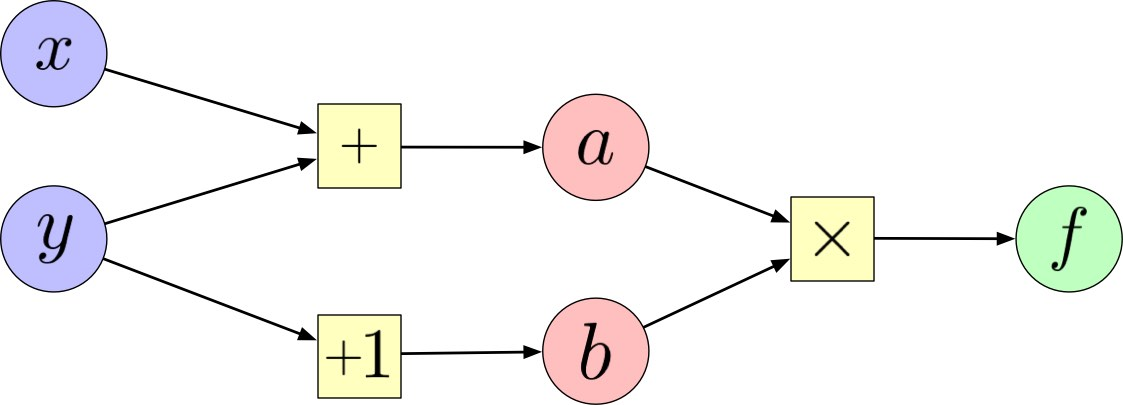
\includegraphics[width=0.5\textwidth]{assets/comp_graph_example.jpg}
    \caption{}
    \label{fig:comp_graph_example}
\end{figure}

We can then work backwards and compute the derivative of $f$ w.r.t. each
intermediate variable ($\frac{\del f}{\del a}$, $\frac{\del f}{\del b}$) and
chain them together to get $\frac{\del f}{\del x}$ and $\frac{\del f}{\del y}$. \\

Let $\sigma(\cdot)$ denote the standard sigmoid function. Now, for the following vector function:

\begin{align}
f_1(w_1, w_2) &= \cos(w_1)\cos(w_2) + \sigma(w_2) \\
f_2(w_1, w_2) &= \ln(w_1 + w_2) + w_1^2 w_2
\end{align}

\begin{enumerate}
\item Draw the computation graph (you might find \href{https://draw.io/}{draw.io} useful for this). Compute the value of $f$ at $\vec{w} = (1, 2)$.
\item At this $\vec{w}$, compute the Jacobian $\frac{\del \vec{f}} {\del \vec{w}}$ using numerical differentiation (using $\Delta w$ = 0.01).
\item At this $\vec{w}$, compute the Jacobian using forward mode auto-differentiation.
\item At this $\vec{w}$, compute the Jacobian using backward mode auto-differentiation.
\item Don't you love that software exists to do this for us? \textit{ungraded :)}
\end{enumerate}

\paragraph{Solution:}

\textbf{(a) Computation Graph and Evaluation of $\vec{f}(1, 2)$:}

We define the elementary intermediate variables in the computation graph as follows:
\begin{align*}
    v_{-1} &= w_1 = 1 \\
    v_{0} &= w_2 = 2 \\
    v_1 &= \cos(v_{-1}) = \cos(1) \approx 0.540302 \\
    v_2 &= \cos(v_0) = \cos(2) \approx -0.416147 \\
    v_3 &= v_1 \times v_2 = \cos(1)\cos(2) \approx -0.224845 \\
    v_4 &= \sigma(v_0) = \frac{1}{1 + e^{-2}} \approx 0.880797 \\
    v_5 &= v_3 + v_4 = f_1(w_1, w_2) \approx 0.655952 \\
    v_6 &= v_{-1} + v_0 = w_1 + w_2 = 3 \\
    v_7 &= \ln(v_6) = \ln(3) \approx 1.098612 \\
    v_8 &= (v_{-1})^2 = w_1^2 = 1 \\
    v_9 &= v_8 \times v_0 = w_1^2 w_2 = 2 \\
    v_{10} &= v_7 + v_9 = f_2(w_1, w_2) \approx 3.098612
\end{align*}

\begin{center}
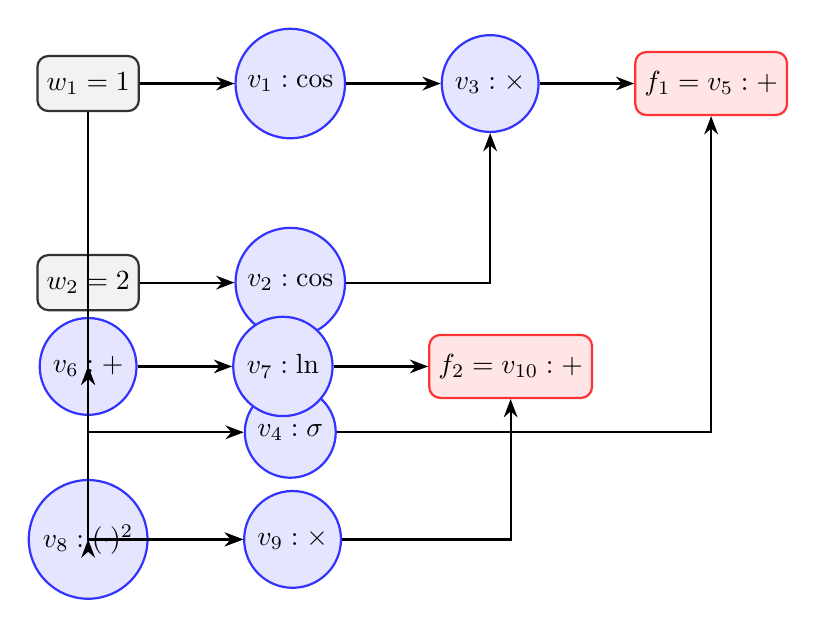
\begin{tikzpicture}[
    node distance=1.2cm and 1.5cm,
    op/.style={circle, draw=blue!80, fill=blue!10, thick, minimum size=8mm},
    var/.style={rectangle, draw=black!80, fill=gray!10, rounded corners, thick, minimum size=7mm},
    outnode/.style={rectangle, draw=red!80, fill=red!10, rounded corners, thick, minimum size=8mm},
    >=Stealth, thick
]
    \node[var] (w1) {$w_1 = 1$};
    \node[var, below=1.8cm of w1] (w2) {$w_2 = 2$};
    
    % f1 branch
    \node[op, right=1.2cm of w1] (cos1) {$v_1:\cos$};
    \node[op, right=1.2cm of w2] (cos2) {$v_2:\cos$};
    \node[op, below=0.6cm of cos2] (sig) {$v_4:\sigma$};
    \node[op, right=1.2cm of cos1] (mult1) {$v_3:\times$};
    \node[outnode, right=1.2cm of mult1] (f1) {$f_1 = v_5: +$};
    
    % f2 branch
    \node[op, below=2.6cm of w1] (sum1) {$v_6:+$};
    \node[op, right=1.2cm of sum1] (ln1) {$v_7:\ln$};
    \node[op, below=0.8cm of sum1] (sq1) {$v_8:(\cdot)^2$};
    \node[op, right=1.2cm of sq1] (mult2) {$v_9:\times$};
    \node[outnode, right=1.2cm of ln1] (f2) {$f_2 = v_{10}: +$};

    % edges
    \draw[->] (w1) -- (cos1);
    \draw[->] (w2) -- (cos2);
    \draw[->] (w2) |- (sig);
    \draw[->] (cos1) -- (mult1);
    \draw[->] (cos2) -| (mult1);
    \draw[->] (mult1) -- (f1);
    \draw[->] (sig) -| (f1);
    
    \draw[->] (w1) |- (sum1);
    \draw[->] (w2) |- (sum1);
    \draw[->] (sum1) -- (ln1);
    \draw[->] (w1) |- (sq1);
    \draw[->] (sq1) -- (mult2);
    \draw[->] (w2) |- (mult2);
    \draw[->] (ln1) -- (f2);
    \draw[->] (mult2) -| (f2);
\end{tikzpicture}
\end{center}

Evaluating the vector function at $\vec{w} = (1, 2)$:
\begin{equation}
    \vec{f}(1, 2) = \begin{bmatrix} f_1(1, 2) \\ f_2(1, 2) \end{bmatrix} = \begin{bmatrix} \cos(1)\cos(2) + \sigma(2) \\ \ln(3) + 1^2 \cdot 2 \end{bmatrix} \approx \begin{bmatrix} 0.655952 \\ 3.098612 \end{bmatrix}
\end{equation}

\vspace{0.5em}
\textbf{(b) Numerical Differentiation ($\Delta w = 0.01$):}

Using forward finite differences with step $\Delta w = 0.01$:
\begin{align*}
    \vec{w} + \Delta w \vec{e}_1 &= (1.01, 2) \\
    f_1(1.01, 2) &= \cos(1.01)\cos(2) + \sigma(2) \approx 0.531843 \times (-0.416147) + 0.880797 = 0.659472 \\
    f_2(1.01, 2) &= \ln(3.01) + (1.01)^2 \cdot 2 \approx 1.101940 + 2.040200 = 3.142140 \\
    \vec{w} + \Delta w \vec{e}_2 &= (1, 2.01) \\
    f_1(1, 2.01) &= \cos(1)\cos(2.01) + \sigma(2.01) \approx 0.540302 \times (-0.425239) + 0.881845 = 0.652079 \\
    f_2(1, 2.01) &= \ln(3.01) + 1^2 \cdot 2.01 \approx 1.101940 + 2.010000 = 3.111940
\end{align*}
Computing each finite-difference quotient:
\begin{align}
    \frac{\partial f_1}{\partial w_1} &\approx \frac{f_1(1.01, 2) - f_1(1, 2)}{0.01} = \frac{0.659472 - 0.655952}{0.01} \approx 0.3520 \\
    \frac{\partial f_1}{\partial w_2} &\approx \frac{f_1(1, 2.01) - f_1(1, 2)}{0.01} = \frac{0.652079 - 0.655952}{0.01} \approx -0.3873 \\
    \frac{\partial f_2}{\partial w_1} &\approx \frac{f_2(1.01, 2) - f_2(1, 2)}{0.01} = \frac{3.142140 - 3.098612}{0.01} \approx 4.3528 \\
    \frac{\partial f_2}{\partial w_2} &\approx \frac{f_2(1, 2.01) - f_2(1, 2)}{0.01} = \frac{3.111940 - 3.098612}{0.01} \approx 1.3328
\end{align}
Thus, the numerically estimated Jacobian is:
\begin{equation}
    \frac{\partial \vec{f}}{\partial \vec{w}} \approx \begin{bmatrix} 0.3520 & -0.3873 \\ 4.3528 & 1.3328 \end{bmatrix}
\end{equation}

\vspace{0.5em}
\textbf{(c) Forward-Mode Automatic Differentiation:}

Forward mode propagates primal values $v_i$ alongside tangent values $\dot{v}_i = \nabla v_i \cdot \dot{\vec{w}}$.
\begin{itemize}
    \item \textbf{Seed 1: $\dot{\vec{w}} = [1, 0]^T$ ($\dot{w}_1 = 1, \dot{w}_2 = 0$):}
    \begin{align*}
        \dot{v}_1 &= -\sin(v_{-1})\dot{v}_{-1} = -\sin(1)(1) \approx -0.841471 \\
        \dot{v}_2 &= -\sin(v_0)\dot{v}_0 = -\sin(2)(0) = 0 \\
        \dot{v}_3 &= \dot{v}_1 v_2 + v_1 \dot{v}_2 = (-0.841471)(-0.416147) + 0 \approx 0.350176 \\
        \dot{v}_4 &= \sigma(v_0)(1-\sigma(v_0))\dot{v}_0 = 0 \\
        \dot{v}_5 &= \dot{v}_3 + \dot{v}_4 = 0.350176 + 0 = 0.350176 \implies \frac{\partial f_1}{\partial w_1} = 0.350176 \\
        \dot{v}_6 &= \dot{v}_{-1} + \dot{v}_0 = 1 + 0 = 1 \\
        \dot{v}_7 &= \frac{\dot{v}_6}{v_6} = \frac{1}{3} \approx 0.333333 \\
        \dot{v}_8 &= 2 v_{-1} \dot{v}_{-1} = 2(1)(1) = 2 \\
        \dot{v}_9 &= \dot{v}_8 v_0 + v_8 \dot{v}_0 = (2)(2) + 0 = 4 \\
        \dot{v}_{10} &= \dot{v}_7 + \dot{v}_9 = \frac{1}{3} + 4 = \frac{13}{3} \approx 4.333333 \implies \frac{\partial f_2}{\partial w_1} = 4.333333
    \end{align*}
    
    \item \textbf{Seed 2: $\dot{\vec{w}} = [0, 1]^T$ ($\dot{w}_1 = 0, \dot{w}_2 = 1$):}
    \begin{align*}
        \dot{v}_1 &= -\sin(1)(0) = 0 \\
        \dot{v}_2 &= -\sin(v_0)\dot{v}_0 = -\sin(2)(1) \approx -0.909297 \\
        \dot{v}_3 &= \dot{v}_1 v_2 + v_1 \dot{v}_2 = 0 + (0.540302)(-0.909297) \approx -0.491295 \\
        \dot{v}_4 &= \sigma(2)(1-\sigma(2))(1) = (0.880797)(0.119203) \approx 0.104994 \\
        \dot{v}_5 &= \dot{v}_3 + \dot{v}_4 = -0.491295 + 0.104994 = -0.386301 \implies \frac{\partial f_1}{\partial w_2} = -0.386301 \\
        \dot{v}_6 &= \dot{v}_{-1} + \dot{v}_0 = 0 + 1 = 1 \\
        \dot{v}_7 &= \frac{\dot{v}_6}{v_6} = \frac{1}{3} \approx 0.333333 \\
        \dot{v}_8 &= 2 v_{-1} \dot{v}_{-1} = 2(1)(0) = 0 \\
        \dot{v}_9 &= \dot{v}_8 v_0 + v_8 \dot{v}_0 = 0 + (1)(1) = 1 \\
        \dot{v}_{10} &= \dot{v}_7 + \dot{v}_9 = \frac{1}{3} + 1 = \frac{4}{3} \approx 1.333333 \implies \frac{\partial f_2}{\partial w_2} = 1.333333
    \end{align*}
\end{itemize}
Thus, the Jacobian computed by forward-mode autodiff is:
\begin{equation}
    \frac{\partial \vec{f}}{\partial \vec{w}} = \begin{bmatrix} 0.350176 & -0.386301 \\ 4.333333 & 1.333333 \end{bmatrix}
\end{equation}

\vspace{0.5em}
\textbf{(d) Backward-Mode Automatic Differentiation:}

Backward-mode propagates adjoints $\bar{v}_i = \frac{\partial f_k}{\partial v_i}$ in reverse topological order.
\begin{itemize}
    \item \textbf{Adjoint Seed 1 for $f_1$ ($\bar{v}_5 = 1, \bar{v}_{10} = 0$):}
    \begin{align*}
        \bar{v}_3 &= \bar{v}_5 \frac{\partial v_5}{\partial v_3} = 1, \quad \bar{v}_4 = \bar{v}_5 \frac{\partial v_5}{\partial v_4} = 1 \\
        \bar{v}_1 &= \bar{v}_3 \frac{\partial v_3}{\partial v_1} = 1 \cdot v_2 = \cos(2) \approx -0.416147 \\
        \bar{v}_2 &= \bar{v}_3 \frac{\partial v_3}{\partial v_2} = 1 \cdot v_1 = \cos(1) \approx 0.540302 \\
        \bar{w}_1 &= \bar{v}_1 \frac{\partial v_1}{\partial w_1} = (-0.416147)(-\sin(1)) \approx 0.350176 \\
        \bar{w}_2 &= \bar{v}_2 \frac{\partial v_2}{\partial w_2} + \bar{v}_4 \frac{\partial v_4}{\partial w_2} = (0.540302)(-\sin(2)) + 1 \cdot \sigma(2)(1-\sigma(2)) \approx -0.491295 + 0.104994 = -0.386301
    \end{align*}
    
    \item \textbf{Adjoint Seed 2 for $f_2$ ($\bar{v}_5 = 0, \bar{v}_{10} = 1$):}
    \begin{align*}
        \bar{v}_7 &= \bar{v}_{10} \frac{\partial v_{10}}{\partial v_7} = 1, \quad \bar{v}_9 = \bar{v}_{10} \frac{\partial v_{10}}{\partial v_9} = 1 \\
        \bar{v}_6 &= \bar{v}_7 \frac{\partial v_7}{\partial v_6} = \frac{1}{v_6} = \frac{1}{3} \\
        \bar{v}_8 &= \bar{v}_9 \frac{\partial v_9}{\partial v_8} = 1 \cdot v_0 = 2 \\
        \bar{w}_1 &= \bar{v}_6 \frac{\partial v_6}{\partial w_1} + \bar{v}_8 \frac{\partial v_8}{\partial w_1} = \frac{1}{3}(1) + 2(2 w_1) = \frac{1}{3} + 4 = \frac{13}{3} \approx 4.333333 \\
        \bar{w}_2 &= \bar{v}_6 \frac{\partial v_6}{\partial w_2} + \bar{v}_9 \frac{\partial v_9}{\partial w_2} = \frac{1}{3}(1) + 1(v_8) = \frac{1}{3} + 1 = \frac{4}{3} \approx 1.333333
    \end{align*}
\end{itemize}
Thus, backward-mode autodiff produces the exact same Jacobian:
\begin{equation}
    \frac{\partial \vec{f}}{\partial \vec{w}} = \begin{bmatrix} 0.350176 & -0.386301 \\ 4.333333 & 1.333333 \end{bmatrix}
\end{equation}

\vspace{0.5em}
\textbf{(e) Software reflection:}
Yes! Frameworks like PyTorch and JAX automate this exact reverse-mode accumulation seamlessly across billions of parameters.

\end{enumerate}

\newpage

\section{Paper Review}

The first of our paper reviews for this class comes from a NeurIPS 2019 paper on the topic \textbf{`Weight Agnostic Neural Networks'} by \textbf{Adam Gaier} and \textbf{David Ha} from Google Brain.

The paper presents an interesting proposition that, through a series of experiments, re-examines some fundamental notions about neural networks - in particular, the comparative importance of architectures and weights in a network's predictive performance. 

The paper can be viewed \href{https://arxiv.org/abs/1906.04358}{here}.
There's also a helpful \href{https://weightagnostic.github.io/}{interactive webpage} with intuitive visualizations to help you understand its key concepts better. 

The evaluation rubric for this section is as follows:

\begin{enumerate}[resume]
\item
\textbf{[2 points]}
Briefly summarize the key contributions, strengths and weaknesses of this paper.

\paragraph{Solution:}

\textbf{Summary of Contributions:} 
Gaier and Ha challenge the dominant paradigm that neural network capability stems purely from explicit weight optimization via gradient descent. They introduce \emph{Weight Agnostic Neural Networks} (WANNs)—architectures discovered through topological search (an extension of NEAT) with varied activation functions that perform reinforcement learning tasks (e.g., CartPole, BipedalWalker, CarRacing) and classification (MNIST) using a single, shared, randomly assigned weight value drawn from a discrete range $[-2, 2]$.

\textbf{Strengths:}
\begin{enumerate}[leftmargin=*]
    \item \textbf{Conceptual Insight:} Demonstrates that architectural inductive bias alone can encode functional behaviors prior to any gradient-based weight training, drawing a compelling parallel to innate biological instincts.
    \item \textbf{Synergy with SGD:} Shows that WANN-discovered topologies serve as superior initializations, achieving competitive performance when fine-tuned with standard optimizers.
    \item \textbf{Simplicity \& Thoroughness:} Evaluates diverse RL benchmarks and continuous control tasks across broad weight sweeps with rigorous ablation.
\end{enumerate}

\textbf{Weaknesses:}
\begin{enumerate}[leftmargin=*]
    \item \textbf{Scalability Constraints:} Topological evolution struggles to scale to high-dimensional state spaces and modern deep vision/NLP architectures.
    \item \textbf{Performance Ceiling:} While impressive for shared constant weights, raw performance without weight tuning lags behind standard overparameterized networks trained end-to-end with backpropagation.
\end{enumerate}

\newpage

\item
\textbf{[2 points]}
What is your personal takeaway from this paper? This could be expressed either in terms of relating the approaches adopted in this paper to your traditional understanding of learning parameterized models, or potential future directions of research in the area which the authors haven't addressed, or anything else that struck you as being noteworthy. 

\paragraph{Solution:}

\textbf{Personal Takeaway:}
The central insight of WANNs fundamentally shifts how we view the duality of neural architecture search (NAS) and parameter learning. Traditional deep learning treats architecture as a passive canvas and delegates all representation learning to weight optimization. WANN demonstrates that topology is an active computational inductive bias that encodes strong functional priors—mirroring precocial species born with innate motor skills.

\textbf{Future Directions \& Connections:}
\begin{enumerate}[leftmargin=*]
    \item \textbf{Connection to the Lottery Ticket Hypothesis (LTH):} WANN can be viewed as an evolutionary analogue to finding "winning tickets" where connectivity itself, rather than delicate parameter magnitudes, drives performance.
    \item \textbf{Differentiable Architecture \& Weight Co-Search:} Future work could integrate continuous relaxation of WANN search with gradient-based NAS (DARTS) to simultaneously discover innate topological priors and fine-grained weights.
    \item \textbf{Hardware-Efficient Neuromorphic Computing:} Weight-agnostic topologies could dramatically lower power consumption on edge/analog devices, where storing and retrieving dense floating-point weights is the primary energy bottleneck.
\end{enumerate}

\end{enumerate}

\textbf{Guidelines}: Please restrict your reviews to no more than 350 words (total length for answers to both the above questions).

\end{document}
